\section{union}
\label{sec:union}
\begin{frame}<beamer>
    \frametitle{Outline}
    \tableofcontents[currentsection]
\end{frame}

\begin{frame}[fragile]{union}
\begin{itemize}
	\item {Sometimes it is not necessary to reserve a field for each struct member}
	\item {Several fields are allowed to share the same block of memory}
	\item {This special type of structure is called \textcolor{blue}{union}}
\end{itemize}
\begin{columns}
\begin{column}{0.45\linewidth}
\begin{lstlisting}
struct Data {
   short i;
   float f;
   char str[20];
};
\end{lstlisting}
\end{column}
\begin{column}{0.45\linewidth}
\begin{lstlisting}
union Data {
   short i;
   float f;
   char str[20];
};
\end{lstlisting}
\end{column}
\end{columns}
\end{frame}

\begin{frame}[fragile]{union: definition (1)}
\begin{center}
	\Large{
   \textcolor{blue}{union} [union tag] \{ \\
   \textcolor{blue}{type1} member1; \\
   \textcolor{blue}{type2} member2; \\
   ... \\
   \};
	}
\end{center}
\begin{itemize}
	\item {It is basically very similar as \textcolor{blue}{struct}}
	\item {However, the members are kept in different way}
\end{itemize}
\begin{columns}
\begin{column}{0.45\linewidth}
\begin{lstlisting}
struct Data1 {
   short i;
   float f;
   char str[20];
};
\end{lstlisting}
\end{column}
\begin{column}{0.45\linewidth}
\begin{lstlisting}
union Data2 {
   short i;
   float f;
   char str[20];
};
\end{lstlisting}
\end{column}
\end{columns}
\end{frame}

\begin{frame}[fragile]{union: definition (2)}
\vspace{-0.2in}
\begin{lstlisting}
struct Data1 {
   short i;
   float f;
   char str[10];
};

union Data2 {
   short i;
   float f;
   char str[10];
};
int main()
{
   Data1 d1;
   Data2 d2;
   printf("Size of d1 %d", sizeof(d1));
   printf("Size of d2 %d", sizeof(d2));
   return 0;
}
\end{lstlisting}
\vspace{-0.15in}
[Output:???]
\end{frame}

\begin{frame}[fragile]{union: definition (3)}
\begin{lstlisting}
int main()
{
   Data1 d1;
   Data2 d2;
   printf("Size of d1 %d", sizeof(d1));
   printf("Size of d2 %d", sizeof(d2));
   return 0;
}
\end{lstlisting}
\begin{center}
Size of d1: 20 \\
Size of d2: 12
\end{center}
\begin{itemize}
	\item {Can you figure out why??}
\end{itemize}
\end{frame}

\begin{frame}[fragile]{union: definition (4)}
\begin{lstlisting}
int main()
{
   Data1 d1;
   Data2 d2;
   printf("Size of d1 %d", sizeof(d1));
   printf("Size of d2 %d", sizeof(d2));
   return 0;
}
\end{lstlisting}
\begin{center}
Size of d1: 20 \\
Size of d2: 12
\end{center}
\begin{itemize}
	\item {For the convenience of memory allocation}
	\item {\textcolor{green}{str} will be given \textcolor{red}{12} bytes instead of 10}
\end{itemize}
\end{frame}

\begin{frame}[fragile]{union: how they are kept in the memory}
\begin{figure}
	\subfigure[struct]
	{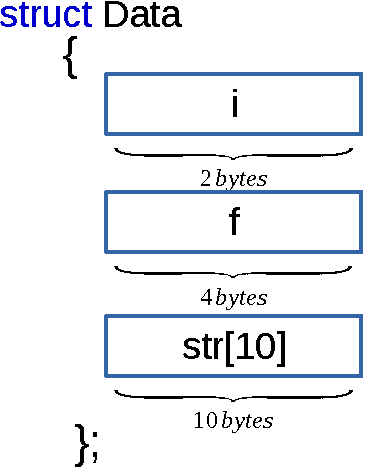
\includegraphics[width=0.25\linewidth]{figs/struct.pdf}}
	\hspace{0.15in}
	\subfigure[union]
	{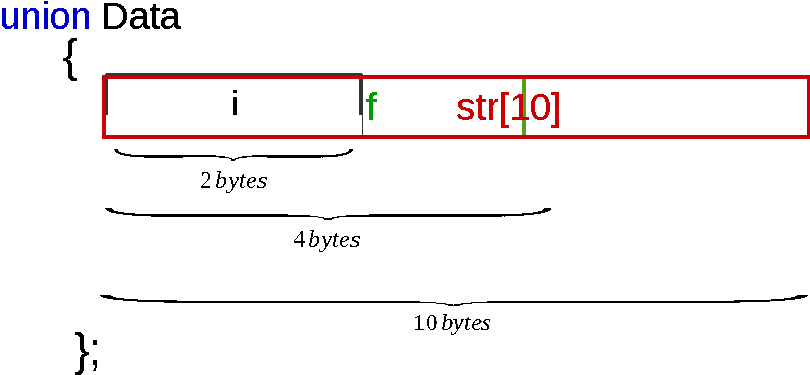
\includegraphics[width=0.6\linewidth]{figs/union.pdf}}
\end{figure}
\end{frame}

\begin{frame}[fragile]{union: learn by example (1)}
\begin{lstlisting}
#include <stdio.h>
#include <string.h>
union Data {
   int i;
   float f;
   char str[20];
};
int main() 
{
   union Data data;        
   data.i = 10;
   data.f = 220.5;
   strcpy( data.str, "C Programming");

   printf( "data.i : %d\n", data.i);
   printf( "data.f : %f\n", data.f);
   printf( "data.str : %s\n", data.str);
   return 0;
}
\end{lstlisting}
\begin{itemize}
	\item {See what the output??}
\end{itemize}
\end{frame}

\begin{frame}[fragile]{union: learn by example (2)}
\vspace{-0.2in}
\begin{lstlisting}
#include <stdio.h>
#include <string.h>
union Data {
   int i;
   float f;
   char str[20];
};
int main(){
   union Data data;        
   data.i = 10;
   data.f = 220.5;
   strcpy( data.str, "C Programming");
   printf( "data.i : %d\n", data.i);
   printf( "data.f : %f\n", data.f);
   printf( "data.str : %s\n", data.str);
}
\end{lstlisting}
\vspace{-0.20in}
data.i : 1917853763\\
data.f : 4122360580327794860452759994368.000000\\
data.str : C Programming
\end{frame}

\begin{frame}[fragile]{union: learn by example (3)}
\vspace{-0.2in}
\begin{lstlisting}
#include <stdio.h>
#include <string.h>
union Data {
   int i;
   float f;
   char str[20];
};
int main(){
   union Data data;        
   data.i = 10;
   strcpy( data.str, "C Programming");
   data.f = 220.5;
   printf( "data.i : %d\n", data.i);
   printf( "data.f : %f\n", data.f);
   printf( "data.str : %s\n", data.str);
}
\end{lstlisting}

\end{frame}

\begin{frame}[fragile]{union: learn by example (4)}
\vspace{-0.16in}
\begin{lstlisting}
#include <stdio.h>
#include <string.h>
union Data {
   int i;
   float f;
   char str[20];
};
int main(){
   union Data data;        
   data.i = 10;
   strcpy( data.str, "C Programming");
   data.f = 220.5;
   printf( "data.i : %d\n", data.i);
   printf( "data.f : %f\n", data.f);
   printf( "data.str : %s\n", data.str);
}
\end{lstlisting}
\vspace{-0.16in}
data.i : 1130135552 \\
data.f : 220.500000 \\
data.str : 
\end{frame}

\begin{frame}[fragile]{union: learn by example (5)}
\vspace{-0.16in}
\begin{lstlisting}
#include <stdio.h>
#include <string.h>
union Data {
   int i;
   float f;
   char str[20];
};
int main(){
   data.i = 10;
   printf( "data.i : %d\n", data.i);
   data.f = 220.5;
   printf( "data.f : %f\n", data.f);
   strcpy( data.str, "C Programming");
   printf( "data.str : %s\n", data.str);
}
\end{lstlisting}

\end{frame}

\begin{frame}[fragile]{union: learn by example (6)}
\vspace{-0.16in}
\begin{lstlisting}
#include <stdio.h>
#include <string.h>
union Data {
   int i;
   float f;
   char str[20];
};
int main(){
   data.i = 10;
   printf( "data.i : %d\n", data.i);
   data.f = 220.5;
   printf( "data.f : %f\n", data.f);
   strcpy( data.str, "C Programming");
   printf( "data.str : %s\n", data.str);
}
\end{lstlisting}
\vspace{-0.16in}
data.i : 10 \\
data.f : 220.500000 \\
data.str : C Programming
\end{frame}


